\chapter{Antecedentes}
	\section{Robots bípedos}
		\subsection*{Conceptos básicos}
Un robot con piernas es un robot móvil que debe tener un cuerpo, al menos una pierna (extremidad inferior) y un número arbitrario de brazos (extremidades superiores). Generalmente sus piernas deben tener un actuador final con el cual apoyarse e impusarse  y sus brazos, un actuador para manipular objetos \citep{siciliano2016springer}. Por lo tanto, se puede deducir que un \textit{robot bípedo} es un robot con dos piernas las cuales usa para moverse, de forma similar al caminado.
\\

Entre los \textit{robots bípedos} más conocidos se encuentran los \textit{robots humanoides} (figura \ref{fig:humanoids}) que poseen las siguientes características[]:

\begin{itemize}
\item Tienen la apariencia y forma de un ser humano, por lo que su cuerpo debe consistir de dos brazos, dos piernas y una cabeza ajustada a un tronco.
\item Deber ser capaces de permanecer de pie sobre sus pies y caminar con sus piernas.
\item Pueden interactuar con humanos usando reconocimiento de voz y/o de imágenes.
\item Los movimientos que son capaces de hacer deben ser cinenmáticamente equivalentes a los de un ser humano por ejemplo, las articulaciones de la rodilla no deben doblarse para atrás, la cabeza no debe girar a más de 180 grados, ni debe tener actuadores lineales en sus extremidades.
\end{itemize}

Uno de los mayores retos a la hora de diseñar y modelar a los robot bípedos es su movimiento. A comparación de otros robots móviles, los robots con piernas tienden a tener un mayor número de grados de libertad en sus extremidades y estos deben estar muy bien coordinados para no hacer caer al robot. 
\\
			\subsubsection*{Características para el diseño de un robot con piernas}
\begin{itemize}
\item \textbf{Tipo de marcha:} Es el patrón de movimientos de piernas del robot (caminata).

\item \textbf{Biomímesis:} Es el diseño de algunos robots para imitar la estructura mecánica de un ser vivo de tal manera que sea tan precisa como se pueda.

\item \textbf{Bioinspiración mecánica:} Es el diseño que sirve para reproducir la robustez y versatilidad de la locomoción de animales, algunos diseñadores prestan más atención en la dinámica esencial de la locomoción que en la mecánica.

\item \textbf{Simplicidad mecánica:} Con esto se pretende usar el menor número de actuadores posibles para cumplir sólo con las tareas realizadas.

\item \textbf{Espacio de trabajo de la extremidad: } Señala que una extremidad debería tener al menos 3GDL para moverse libremente en el espacio. Para que se pueda tener una arbitraria orientación en el efector final en un espacio 3-D se debe contar con almenos 6GDL.

\end{itemize}

\begin{figure}
	\centering		
	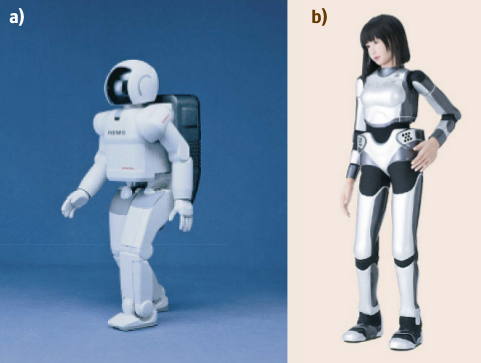
\includegraphics[scale=0.5]{images/asimov_and_HRP-4C.png}
	\caption{Ejemplos de robots humanoides (a) Asimov (2000); (b)HRP-4C (2009) (Tomado de: Siciliano and Khatib, 2016).}		
\label{fig:humanoids}%(Ver página 423).
\end{figure}


			\subsubsection*{Análisis de estabilidad}

Para el control del sistema dinámico no lineal hay  un número de conceptos relativos para su seguridad y estabilidad:

\begin{itemize}
\item \textit{Puntos fijos} : Representan las posturas estáticas en cuáles el robot puede estar de pie de manera segura.

\item \textit{Ciclos límites}: Proveen una natural extensión del análisis de los puntos fijos para movimientos de caminata periódica.

\item \textit{Viabilidad}: La viabilidad es un concepto de invarianza controlada, que analiza el conjunto de estados del cual el robot es capaz de mantenerse de pie. Desafortunadamente esta propiedad puede ser intratable para el cómputo.

\item \textit{Controlabilidad}: La controlabilidad provee una ligera noción de restricción de viabilidad, analizando el conjunto de estados del cual el robot es capaz de retornar a un particular punto fijo.

\item \textit{Estabilidad robusta}: Examina las propiedades del sistema considerando el "peor de los casos" de las perturbaciones. Por instancias, un controlador robusto debería ser capaz de garantizar que un punto fijo es estable incluso si la estimación de masa del tronco tiene un error del $\pm$10\%.

\item \textit{Estabilidad estocástica}: El análisis estocástico provee herramientas para investigar la probabilidad de caer. Para muchos modelos de perturbaciones en robots el sistema caerá eventualmente (con probabilidad uno), pero el análisis puede revelar la distribución del tiempo de vida metaestable.

\item \textit{Estabilidad de entrada-salida}: En este análisis se trata una particular perturbación como una entrada, un criterio de rendimiento como salida e intenta calcular una ganancia relativa o sensibilidad del rendimiento del robot debido a esta entrada.

\item \textit{Márgenes de estabilidad}: El análisis de robustez puede ser difícil. En la práctica, los diseñadores del control a menudo se conforman con que el sistema se mantenga cómodamente lejos de los límites de estabilidad determinista.		

\end{itemize}

	\section{Aplicaciones en el juego de Futbol Soccer}	
		\subsubsection*{Futbol Soccer en el concurso RoboCup}
		La \textit{RoboCup} es una internacional iniciativa para promover la inteligencia artificial y la tecnología robótica a través de la organización de competencias y encuentros científicos. Una de las categorías más famosas dentro de este concurso es el de robots humanoides para soccer (Humanoid League) cuyo objetivo es lograr que para la mitad del siglo XXI un equipo de robots humanoides autónomos sean capaces de ganar una partida de fútbol contra el recien campeón mundial de ese entonces, siguiendo las reglas oficiales de la FIFA.
		
		La categoría de soccer comenzó en el año de 1997 con simples y simulados robots con ruedas, desde entonces el desarrollo  fue creciendo hasta que en el 2002 se inició la liga de humanoides cuyos principales retos eran los comportamientos como caminar, patear y percibir el ambiente. Desde entonces, año con año las mejoras en los mecanismos, la electrónica y control han hecho evolucionar el desarrollo para que la \textit{biomímesis} sea la más parecida a la de un humano.\citep{gerndt2015humanoid}
		
		\subsubsection*{Liga de robots humanoides de categoría \textit{TeenSize}}
		En los recientes años, la introducción de robots estandarizados, accesibles y de bajo costo ha tenido un formidable impacto para la creación y desarrollo de robots de soccer. Un ejemplo es el humanoide \textit{DARwIn-OP} (Figura \ref{fig:Darwin_OP}) que se organiza dentro de la categoría \textit{KidSize}. De esta manera, algunos comportamientos del soccer ya están implementados, de modo que los investigadores tienen la oportunidad de enfocarse en tareas de más alto nivel. \citep{schwarz2013humanoid}
		
		A pesar que \textit{DARwIn-OP} ha facilitado que los equipos lleguen a tener el número necesario de jugadores, no es lo mismo para otras categorías en donde los robots tienden a tener mayor tamaño (como en \textit{TeenSize} o \textit{AdultSize}) no se llega a tener el número deseado de jugadores y algunos competidores se ven forzados a participar con robots hechos por ellos mismos. Consecuentemente esto altera el desempeño de los partidos y retraza el desarrollo de nuevos comportamientos. Para solucionar este problema fue desarrollado un primer prototipo de plataforma abierta basado el \textit{Darwin-OP} para la categoría \textit{TeenSize} llamado \textit{Nimbro-OP} (véase la sección 5.1) el cual tiene un diseño de fácil manufactura, ensamblaje y mantenimiento.	 

\begin{figure}
\centering
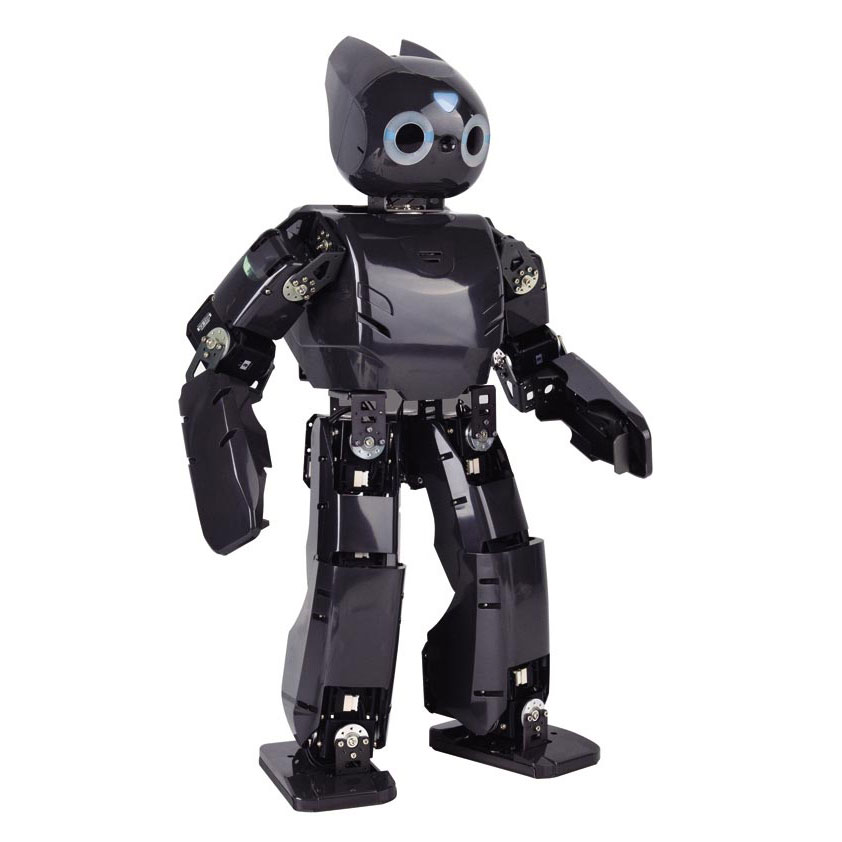
\includegraphics[scale=0.25]{images/Darwin_OP.jpg}
\caption{Robot Humanoide Darwin-OP}
\label{fig:Darwin_OP}
\end{figure}

	\section{Usos de la visión computacional}
		\subsection*{Precedentes }
	A falta de sistemas de visión para el reconocimiento y localización de objetos en misiles no tripulados durante la Segunda Guerra Mundial, la industria bélica norteamericana llegó financiar la investigación para misiles teleoperados por palomas (Figura \ref{fig:project_pigeon}a), siguiendo las nacientes investigaciones sobre el Condicionamiento Operante de B.F. Skinner. Este proyecto se llamó \textit{Project Pigeon}  \citep{capshew1993engineering} y consisitía en meter palomas dentro de misiles para que estas picotearan la imagen en donde aparecían los barcos en medio del mar, véase la Figura \ref{fig:project_pigeon}b.

\begin{figure}
\centering
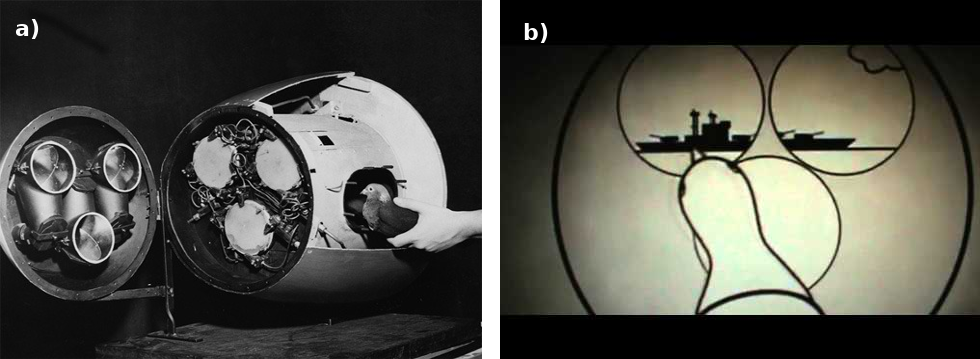
\includegraphics[scale=0.3]{images/project_pigeon.png}
\caption{(a) \textit{Proyecto Pigeon} para teleoperación de misiles de guerra; (b) Condicionamiento de palomas para la dirección de los misiles.}
\label{fig:project_pigeon}
\end{figure}

	A pesar de lo ingenioso e innovador de este proyecto, las fuerzas armadas norteamericanas optaron por abandonarlo para no retrazar otros cuyas aplicaciones eran más prometedoras. 
		
		\subsection*{Visión computacional}
	La \textit{visión computacional} es la transformación de datos desde una imagen o video cámara hacia una \textit{nueva representación} para lograr un fin en particular \cite{bradski2008learning}. Al decir esto, significa que se pueden usar ciertas características de la luz capturada en una imagen (o secuencia de imágenes) para transformarlas en variables numéricas que la computadora pueda abstraer y procesar (tómese de ejemplo la figura \ref{fig:camera_representation}).

\begin{figure}
\centering
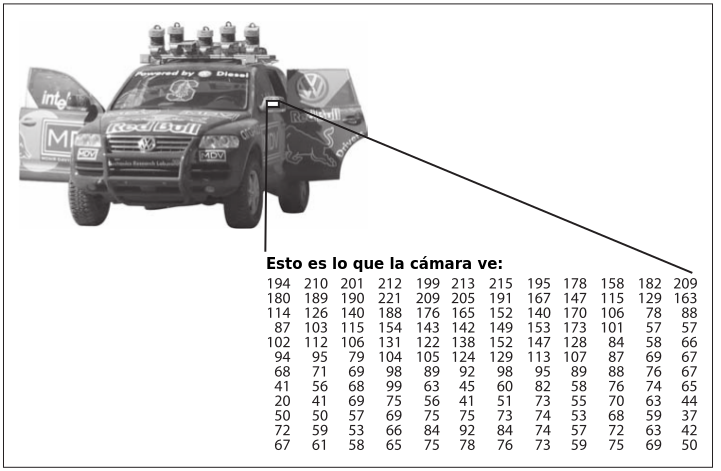
\includegraphics[scale=0.6]{images/new_representation_image.png}
\caption{Representación de cómo una imagen es representada por la computadora. Imagen modificada de:}
\label{fig:camera_representation}
\end{figure}

Para los fines de este trabajo solamente se utilizarán funciones para segmentar objetos con base en su color, para obtener la posición del objeto en el espacio se hizo el análisis matemático de la sección 4.1.
	
	\section{El Filtro de Kalman}
		\subsection*{Filtro de Kalman Discreto}
	En 1060 Rudolf Emil Kalman publicó su famoso \textit{paper} en donde describe una recursiva solución para el problema del filtrado de datos discretos. Desde ese entonces el filtro ha sido sujeto de extensas investigaciones y aplicaciones en la ingeniería.

	El Filtro de Kalman es un conjunto de ecuaciones matemáticas que proveen un eficiente método computacional para estimar el estado de un proceso, de modo que minimiza el error producido por el ruido. Este filtro es una poderosa herramienta en varios aspectos tales como la estimación del pasado, presente y futuro, incluso es capaz de precisar el modelo de un sistema cuya naturaleza es desconocida.
	
		\subsection*{Proceso de estimación}
		El Filtro de Kalman aborda el problema de tratar de estimar el estado $x \in \Re^n$ de un proceso de tiempo discreto que es modelado con la ecuación diferencial \ref{eq:kalman_filter}.
		
\begin{equation}
x_k = Ax_{k-1} + Bu_{k-1}+w_{k-1}
\label{eq:kalman_filter}
\end{equation}

En donde $A$ es una matriz de nxn que relaciona el estado anterior $k-1$ con el estado presente $k$. $B$ es una matriz de $nx1$ que relaciona la entrada de control opcional $u \in R^1$ al estado $x$. 
La medición $z \in \Re^m$, también conocida como matriz de observación se puede modelar con la ecuación \ref{eq:measurement_equation}:

\begin{equation}
z_k = Hx_k+v_k
\label{eq:measurement_equation}
\end{equation}

En \ref{eq:measurement_equation} $H$ es una matriz de $mxn$ que relaciona el estado con la medición $z_k$.  Las variables aleatorias $w_k$ y $v_k$ representan el ruido del proceso y de la medición (respectivamente), asumiendo que son independientes una de la otra. Las expresiones en \ref{eq:normal_distribution_w} y \ref{eq:normal_distribution_R} representan su distribucion normal.

\begin{equation}
p(w) \sim N(0,Q),
\label{eq:normal_distribution_w}
\end{equation}
\begin{equation}
p(w) \sim N(0,R)
\label{eq:normal_distribution_R}
\end{equation}

Con el objetivo de encontrar una ecuación que calcule una estimación \textit{a posteriori} de un estado $\hat{x}_k$ como una combinación lineal de un estado \textit{a priori} $\hat{x}_k^-$ y una proporcional diferencia de una medición actual $z_k$ con una medición de la predicción $H\hat{x}_k^-$ se emplea la ecuación \ref{eq:posteriori_predicted}.

\begin{equation}
\hat{x}_k = \hat{x}_k^- + K(z_k-H\hat{x}_k^-)
\label{eq:posteriori_predicted}
\end{equation}

La diferencia $(z_k-H\hat{x}_k^-)$ dentro de la ecuación \ref{eq:posteriori_predicted} es llamada \textit{innovación} o \textit{residuo}. $K$ es una matriz de $nxm$ que representa la ganancia que reduce el error de covarianza \textit{a posteriori}. Esta ganancia está dada por la ecuación \ref{eq:k_gain}.

\begin{equation}
K_k = P_k^-H^T(HP_k^-H^T+R)^{-1} = \frac{P_k^-H^T}{HP_k^-H^T+R}
\label{eq:k_gain}
\end{equation}

De esta manera, cuando el error de covarianza en la medición $R$ se aproxima a cero, la ganancia $K$  tiene un mayor peso en la ecuación. Por el contrario, cuando el error de covarianza \textit{a posteriori} $P_k^-$ se aproxima a cero, la ganancia $K$ obtiene menor peso. 

Otra forma de entender la utilidad de la ganancia de $K$ es pensar que mientras la ganancia de aproxime a 1, hará que la medición sea más \textit{confiable}, cuando las mediciones se aproximen a cero, serán menos confiables y se tomará como confiable los datos relacionados con el modelo matemático.
		\subsubsection{Algoritmo de filtrado}
El algoritmo consta de dos fases, la fase \textit{predictiva} y la fase \textit{correctiva}. La fase predictiva consta de utilizar un modelo matemático para obtener las posibles mediciones de un fenómeno. La fase correctiva obtiene los valores de la medición y las compara con las obtenidas con el modelo matemático, de manera que se obtienen los valores de salida, tal y como se observa en la figura \ref{eq:kalman_filter}.

\begin{figure}
\centering
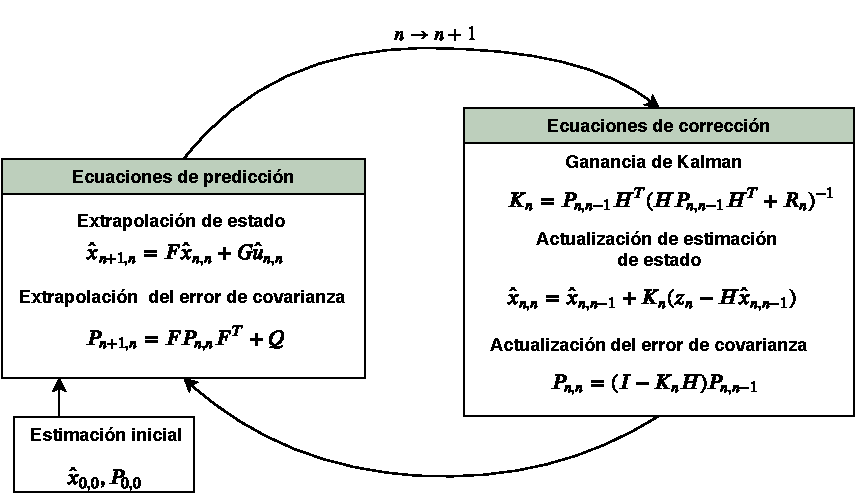
\includegraphics[scale=0.7]{images/kalman_algorithm.pdf}
\caption{Esquema ilustrativo del Filtro de Kalman}
\label{fig:Kalman_scheme}
\end{figure}

	\section{Trabajo relacionado}
		\subsubsection{Percepción del color}
	Una de las técnicas más comunes y prácticas para realizar la detección de objetos para un robot Nimbro-OP es la segmentación por color, es por eso que es muy conveniente que los balones de fútbol en las competencias RoboCup tengan un color diferente al piso en donde descanzan (que generalmente es verde). No obstante, el balón elegido por la comunidad puede tener diferentes matices, por lo que se deben emplear sistemas de aprendizaje para que el robot distinga un balón de cualquier color. 
	
	Tal y como hizo el robot \textit{Dynaped} en 2012 \citep{missura2012robocup}, se obtienen ciertos parámetros de color del tapete usado en la cancha,  para poder encerrar en un contorno el color que no coincida. Véase la figura \ref{fig:ball_contour_1}.
	
\begin{figure}
\centering
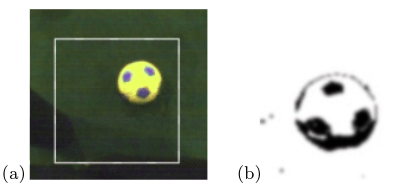
\includegraphics[scale=0.7]{images/ball_contour_1.png}
\caption{(a) Región de interés con un balón desconocido; (b) Segmentación del objeto.}
\label{fig:ball_contour_1}
\end{figure}

	De acuerdo con \citep{behnke2006see} para este tipo de robots, la única fuente de información sobre el ambiente es la cámara, de modo que es conveniente que se disponga de una o más cámaras dentro o fuera del robot. Con una correcta configuración de cámaras se pueden obtener más parámetros del ambiente, tales como posicionamiento del robot, distancia con el objeto de interés, cercanía con otros robots y detección de obstáculos. 
	
	
	
	
	
	
	
	